\section{Design}
\label{s:design}
\hspace{10pt} This section describes the design of the software components and experiments involved in this dissertation. The first subsection outlines how energy demands of different sensors are compared. This includes the design principles behind sample sensor applications and the details on how to measure their energy efficiency. The second subsection lays out the design of the energy-efficient sensing library, Locy. It summarizes its energy-efficient algorithm, how the algorithm can be differentiated depending on battery life and the library's architecture. The design presented in this section will be revisited in the next section.

\subsection{Sensor energy measurements}
\label{s:design:measurements}
\hspace{10pt} Sensor energy measurements are a the part of the project, where the energy efficiencies of different sensors are determined. To achieve this objective, each sensor is represented in a series of simple Android applications, \textbf{Sample Sensor Applications}. Each of these applications continuously samples one sensor and switches off all others. Sample Sensor Applications are designed such that the only one difference between them is which sensor is being sampled. To compare sensors' energy demands, a novel method of measuring energy efficiency of the applications is proposed. The method calculates time each application needs to deplete one percent of battery life. The order of energy efficiency of different sensors may be established by comparing those time measurements: the most energy efficient sensor is the one for which one percentage battery depletion takes longest. 

\subsubsection{Sample sensor applications}
\label{s:design:measurements:sampleapps}
\hspace{10pt} To determine differences in sensors' energy efficiency, each sample applications samples only one sensor while all others sensors are switched off. However, \textbf{this triggers other differences between applications}: various sampling frequencies and sizes of sensor data. Since the aim is to compare the energy efficiency of the sampling itself, the the other differences' impact has been minimized where possible. 

\textbf{Sampling frequencies vary among sensors}. Inertial sensors e.g., accelerometer or gyroscope could be sampled as often as every 20 milliseconds, whereas the minimum frequency of GPS is 20 seconds. The issue is more complex with wireless communication sensors such as Bluetooth or IEEE 802.11. A full Bluetooth scan takes around 12 secs, but could be stopped earlier and restarted. To account for those differences, \textbf{the least energy-efficient strategy of complete, correct sampling} was chosen for comparing sensors' energy efficiency. Sensors are sampled as often as possible, providing the previous sample delivered valid data. For example, the next IEEE 802.11 scan is started once the previous one has finished\ (IEEE 802.11 scan takes around 2.5 secs depending on the device). This provides complete information on available access points, while minimizing sampling frequency, which increases energy consumption. The strategy will look similar for GPS and Bluetooth. Because other sensors' (inertial sensors, camera and microphone) sampling is immediate, they are sampled as often as possible.

To check whether the Sample Sensor Applications work correctly, each application prints out its raw sensor data. The frequency of this output is 1 per second and is constant across applications. As the previous paragraph describes, sensors' data are delivered at different frequencies. Raw data being printed at different frequencies could add noise to our experiments. By using \textbf{the same raw data printing frequency for all applications}, the differences in sampling frequency are mitigated. The GPS sample application prints out its raw sensor data as often as accelerometer sample application, even though they have different sensor sampling frequencies. It is worth noticing that as a side effect, printed values may be repeated or missing, when no new sensor data was delivered in the print interval. 

Another issue concerning applications' output is that \textbf{sensors have different raw data sizes}. For example, the result of wireless communication scans\ (IEEE 802.11 and Bluetooth) consist of a list of records (e.g., 20 access points with their names and other parameters), while a light sensor's result is a single number. Furthermore, more complex data is delivered by the camera and microphone. As the raw data is printed on a regular basis, such differences could lead to significant changes in energy efficiency of the Sample Sensor Applications. To alleviate those differences, \textbf{the output is standardized} to the same form for all applications. One line of output, including between 1 and 3 numbers, is printed.

Those numbers may represent different information depending on the sensor:
\begin{itemize}
	\item For wireless communications sensors, only the number of available access points is printed: 
		\plot{output_wifiscan}
	\item For the microphone, the maximum absolute amplitude for every second is printed:
		\plot{output_microphone}
	\item For the camera, the total size of the recorded video is printed:
		\plot{output_camera}
	\item The light and proximity sensor provide only one value:
		\plot{output_light}
	\item Other inertial sensors provide all three coordinates:
		\plot{output_inertial}
\end{itemize}

There are still other issues that could add noise to the experiments e.g., various API among sensors or different capabilities of IEEE 802.11 wireless cards. However, all differences noticeable on the application level are eliminated. Such a design of the Sample Sensor Applications guarantees that the energy efficiencies of different sensors' sampling is compared. 
				
\subsubsection{1\% battery depletion}	
\label{s:design:measurements:method}
\hspace{10pt} Once the Sample Sensor Applications are prepared, they need to be ranked by energy efficiency. To compare their energy efficiencies, time measurements on how long 1\% depletion of battery life are made. Those time measurements are then compared. For any two sensors, if a longer time is needed for 1\% depletion by one of them, that sensor is more energy-efficient. It is worth mentioning that 1\% is used, because it is the precision of the information on battery life that the Android API provides.

\textbf{The method should be accurate if the comparison is made on the same percentage of battery life} e.g., between 99\% and 98\%. Although the battery life is nonlinear, the battery should behave similarly on the same percentage across many runs. Repeated measurements should be similar. Also, time measurements should be brief, enabling accurate online energy measurement. All of these assumptions will be validated in the next section.

For the purpose of this dissertation, this measurement method was directly incorporated into Sample Sensor Applications. Each sample sensor application continuously queries the battery status and the time of 1\% battery depletion is registered. The whole process is exactly the same for all sample sensor applications, hence adding no noise to the experiments.

\subsubsection{The list of sample sensor applications}	
\label{s:design:measurements:applications}
\hspace{10pt} The Table \ref{table:samplesensorapps} consists of the complete list of Sample Sensor Applications created for this project. Beside the Sample Sensor Applications, a couple of supporting applications were implemented:
\begin{itemize}
	\item EnergyMeasurementListSensors - listing all physical sensors available in a mobile phone.
	\item EnergyMeasurementNetwork - determining energy efficiency of Android wireless-based localization.
	\item EnergyMeasurementGPSSatellites - determining energy efficiency of acquiring GPS Satellites' signal without solving navigation equations on a mobile phone.	
\end{itemize}
All of these applications can be found in the \textit{sensors\_energy\_measurement/sample\_apps} directory.
		
\begin{table}[H]
	\centering
    \begin{tabular}{| l | r | }
    \hline
    \textbf{Sensor} & \textbf{Application name} \\ \hline
    Camera & EnergyMeasurementCamera \\ \hline
    Microphone & EnergyMeasurementMicrophone \\\hline
    IEEE 802.11 & EnergyMeasurementWifi80211 \\ \hline
    GPS & EnergyMeasurementGPS \\ \hline
    Bluetooth & EnergyMeasurementBluetooth \\ \hline
    Bluetooth LTE & EnergyMeasurementBluetoothLE \\ \hline
    Accelerometer & EnergyMeasurementAcceleromter \\ \hline
    Gyroscope & EnergyMeasurementGyroscope \\ \hline
    Magnetic Field & EnergyMeasurementMagneticField\\ \hline
    Ambient Light & EnergyMeasurementLight \\ \hline
    Proximity & EnergyMeasurementProximity \\ \hline
    \end{tabular}
    \caption{The complete list of Sample Sensor Applications.}
	\label{table:samplesensorapps}
\end{table}			


\subsection{Locy}
\label{s:design:locy}
\hspace{10pt}Locy is an energy-efficient sensing library for Android phones. It utilizes relations between sensors to provide energy-efficient localization for mobile applications. The relation is between the accelerometer and GPS sensors. The former may be user to check whether a user is moving or not. If a user is not moving, his geographical location\ (GPS coordinates) do not change. Therefore, GPS sampling may be switched off. This operation brings energy savings, since GPS sampling has higher energy demands than accelerometer sampling.

The library has three important features requiring further explanation. First, a movement detection algorithm needs to be carefully designed to accurately check whether a user is moving. Second, this algorithm needs to be energy-efficient itself. This goal is achieved by duty-cycling sampling with a frequency dependent on the device's battery life\ (the Requirement \ref{r:library:adaptive}). Lastly, the software infrastructure of the library needs to be further discussed. Since the library is aimed at being plugged into existing applications\ (the Requirement \ref{r:library:esm}), its API needs to satisfy specific needs. 

\subsubsection{Movement detection algorithm}
\label{s:design:locy:moving}
\hspace{10pt}The movement detection algorithm is based on accelerometer sensor readings. The sensor provides the raw data describing the acceleration of a device in three dimensions\ (x, y, z relative to the device's position). The data is difficult to analyze: the acceleration of a user may be split between the axes in different ways depending on the initial position of a mobile phone. While a user is walking, accelerometer data will be significantly different depending on where a user keeps their mobile phone\ (horizontally in a purse or vertically in trousers pocket). To simplify the analysis, \textbf{the total magnitude} is applied over accelerometer data\ (Equation \ref{e:total_magnitude}). This reduces the dimensionality of the data to one while retaining the information of the user's acceleration. 

\begin{equation}\label{e:total_magnitude}
total\;magnitude = x^2 + y^2 + z^2
\end{equation}

Once the total magnitude over accelerometer data is applied, the accelerometer readings of a user's walking and their staying in one place may be compared\ (the Figure \ref{p:moving:magnitude}). Walking may be characterized by \textbf{the series of peaks}. A user makes a step by lifting up his foot and putting it back on the ground. The other foot moves in a similar pattern. A peak on a graph corresponds to a user's step. If a user is stationary, no peaks are observed. 

\begin{figure}[H]
\centering
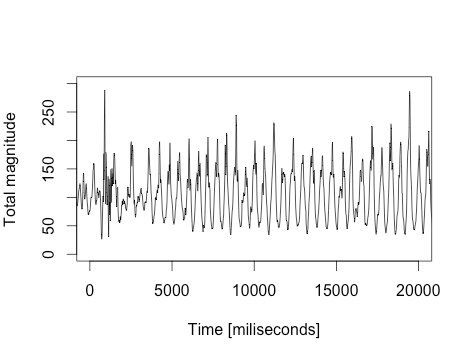
\includegraphics[width=0.49\textwidth, scale=0.6]{plots/walking}
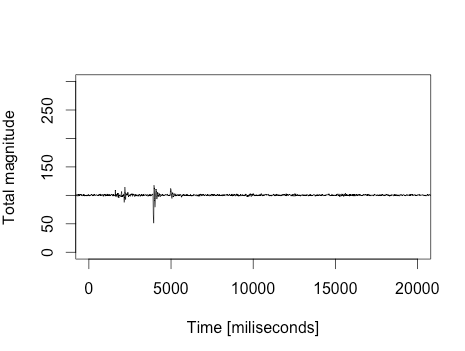
\includegraphics[width=0.49\textwidth, scale=0.6]{plots/no_walking}
\caption{\label{p:moving:magnitude} The difference in total magnitude over accelerometer data between walking and not walking. Walking may be characterized by the series of peaks. One peak corresponds to  a step made by a user.}
\end{figure}

For the purpose of Locy, the difference between walking and being stationary needs to be formalized. While a user is walking, the series of peaks means high accelerometer data variation, which can be expressed by \textbf{standard deviation}. The Figure \ref{p:moving:stddev} contrasts the standard deviation while a user is walking and when they are not\ (a standard deviation was calculated over 2.5 seconds intervals). The standard deviation is much bigger when the user is walking.

\begin{figure}[H]
\centering
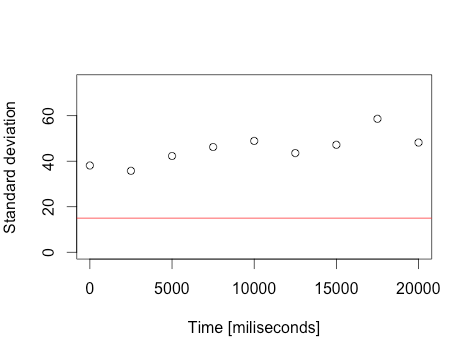
\includegraphics[width=0.49\textwidth, scale=0.6]{plots/stddev_walking}
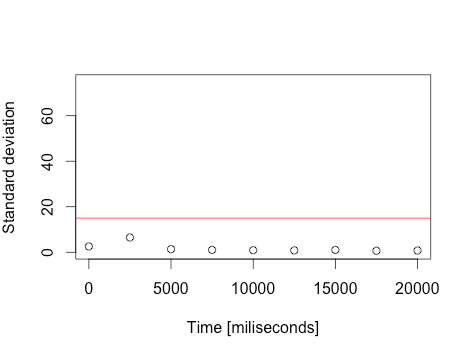
\includegraphics[width=0.49\textwidth, scale=0.6]{plots/stddev_no_walking}
\caption{\label{p:moving:stddev} The difference in standard deviation over total magnitude of accelerometer data between walking and not walking. Walking is characterized by higher standard deviation. The threshold of 15 is chosen to classify a user's movement.}
\end{figure}

There are two challenges with this approach. First, the duration of sampling windows\ (the interval over which a standard deviation is calculated) needs to be chosen. The Figure \ref{p:moving:stddev} uses 2.5 seconds as the duration of sampling windows. Second, the threshold of the standard deviation for the movement classification needs to be determined. The Figure \ref{p:moving:stddev} defines the threshold as 15. Both parameters were determined by \textbf{trial-and-error}. Different values were chosen and evaluated against the small data set collected for the purpose of this project. The best accuracy was provided by the parameters used in the Figure \ref{p:moving:stddev} i.e. 2.5 seconds for sampling windows and 15 as the threshold for movement classification. Details of this trial-and-error approach are presented in the section \ref{s:implementation:moving}.

Locy provides accurate movement detection by undertaking the classification over three consecutive sampling windows. If at least two of them indicates the user is walking\ (the standard deviation is above the threshold), the user activity is classified as walking. Three consecutive sampling windows last in total 7.5 seconds\ (the duration of the sampling window is 2.5 seconds). It is assumed that such a movement detection algorithm is accurate and should be universal i.e. it does not dependent on mobile phone type, position or user.

\subsubsection{Adaptive duty-cycling sampling}
\label{s:design:locy:adaptive}
\hspace{10pt}A user is unlikely to change their activity\ (moving or not) every 8 seconds. This observation could be leveraged for energy optimization. Instead of continuously sampling and classifying accelerometer data, the device could sleep for a certain period of time, conserving energy. After this sleeping interval, the device could start sampling again. This approach is called \textbf{duty-cycling} and is incorporated in Locy. 

Duty-cycling sampling may be customized by changing the \textbf{duty-cycling ratio} between sampling and sleeping window  durations. For example, a ratio of 0.5 means that the duration of sampling windows is half the duration of the sleeping intervals. There is an \textbf{energy-accuracy trade-off} in choosing the ratio: If the ratio is smaller, the important events are more likely to be missed as sampling windows are relatively shorter. On the other hand, smaller ratio leads to bigger energy optimization as the sleeping intervals are relatively longer. Locy utilizes this trade-off by changing its duty-cycling ratio depending on the device's \textbf{remaining battery life}. If the level of battery life is high, the duty-cycling ratio is also high. In that case, Locy does not miss any important events, but is less energy-efficient. If the level of battery level decreases, Locy also decreases its duty-cycling ratio, resulting in additional energy savings. Such an approach satisfies one of the project's secondary requirements\ (the Requirement \ref{r:library:adaptive}). The details of how the ratio changes are presented in the Table \ref{table:locy:dutycyclingratio}.

\begin{table}[H]
	\centering
    \begin{tabular}{| c | c | }
    \hline
    Battery life & Duty-cycling ratio \\ \hline
    80-100\% & 1 \\ \hline
    60-80\% & 0.5\\ \hline
    40-60\% & 0.33\\ \hline
    20-40\% & 0.25\\ \hline
    0-20\% & 0.2 \\ \hline
    \end{tabular}
    \caption{The different duty-cycling ratios in Locy depending on the battery life of a device. Locy adopts its algorithm depending on a current battery life. }
	\label{table:locy:dutycyclingratio}
\end{table}	

\subsubsection{Software architecture}
\label{s:design:locy:architecture}
\hspace{10pt}Locy is an Android library project intended to be plugged into existing applications. Most of those applications use localization services provided by Android's LocationManager. Developers wishing to replace LocalizationManager with Locy should have few difficulties: Locy's API is consistent with the LocationManager API. To use Locy, a developer only needs to add the Locy library to an existing project and change one line in his source code: Instead of getting LocationManager\ (Listing\ref{ls:locationmanager}), LocyManager needs to be created\ (Listing \ref{ls:locymanager}). All other parts of the code should work perfectly without additional changes. This approach was tested by plugging Locy into Tristan's Experience Sampling Method\ (ESM) mobile application. This primary requirement\ (the Requirement \ref{r:library:esm}) was achieved without difficulty. Its results may be viewed in the \textit{ESM/} directory.

                 
\begin{lstlisting}[language=Java,
       basicstyle=\ttfamily,
       keywordstyle=\color{blue}\ttfamily,
       stringstyle=\color{red}\ttfamily,
       commentstyle=\color{green}\ttfamily,
      breaklines=true,
      frame=single,    
      label=ls:locationmanager,caption=Localization services with LocationManager.]
LocationManager locationManager =  (LocationManager) getSystemService(LOCATION_SERVICE);
\end{lstlisting}

\begin{lstlisting}[language=Java,
       basicstyle=\ttfamily,
       keywordstyle=\color{blue}\ttfamily,
       stringstyle=\color{red}\ttfamily,
       commentstyle=\color{green}\ttfamily,
      breaklines=true,
      frame=single,    
      label=ls:locymanager,caption=Localization services with LocyManager.]
LocyManager locationManager = new LocyManager(this);
\end{lstlisting}

